\relatorio{Faixa Azul e segurança viária}
    {
    
      \noindent \textit{working paper}

      \noindent Pesquisadores: Gustavo Theil, Esdras Gomes, Júlio Mugnol e Carlos Cabral

      \noindent Orientado por: Adriano Dutra Teixeira

      \noindent Um projeto em colaboração com Falconi

    }
    {
        Com o objetivo de melhorar a segurança viária na cidade de São Paulo, a CET implementou uma motofaixa exclusiva na Avenida dos Bandeirantes, que ao segregar os usos da via, pretendeu diminuir os conflitos de trânsito e levar a um cenário de tráfego mais seguro. Caso bem sucedida, a medida será implementada em diversos outros trechos da cidade. A teoria microeconômica indica que, apesar de poder haver uma melhora na segurança viária, os motoristas passam a ser menos cautelosos, causando efeitos adversos. Para testar o efeito resultante, utilizou-se o método de controle sintético. Desde a sua inauguração, em outubro de 2022 até dezembro de 2023, estima-se que foram evitados 32 sinistros que envolveriam motociclistas e ao menos uma pessoa ferida de forma grave ou leve, o que representa uma redução de 26.8\% dos sinistros com este perfil registrados no período pós tratamento. Os resultados apresentam robustez com p-valor de 1.35\%.
    }
    {Segurança viária, motofaixa, faixa azul, controle sintético}

\section{Introdução}


De acordo com a Secretaria de Vigilância em Saúde, ``acidentes de trânsito'' são a segunda principal causa de óbito no Brasil para pessoas entre 15 e 49 anos. Na literatura de segurança viária, o termo acidente não é empregado, visto que subentende uma ocorrência inesperada e não intencional. O termo sinistro é considerado mais adequado, pois reconhece a responsabilidade que os agentes de trânsito apresentam para impedir situações envolvendo danos físicos ou materiais \cite{nbr10697}.

Ao redor do planeta, diversas medidas para segurança viária são adotadas, algumas universalmente, outras com cunho experimental e pequena escala. \textcite{wang2013effect} qualificam dois principais fatores que interferem no risco de sinistro: engenharia e comportamento. Sinalização, iluminação, visibilidade, air bags e freio ABS são alguns dos fatores de engenharia que contribuem para a segurança no trânsito. A qualificação do motorista, seu nível de atenção ou se está alcoolizado são exemplos de componentes comportamentais determinantes para o risco de sinistro.

No Brasil, diversas instituições compartilham da responsabilidade de garantir o Art. 1 \S 2 do Código de Trânsito Brasileiro (CTB): ``O trânsito, em condições seguras, é um direito de todos e dever dos órgãos e entidades componentes do Sistema Nacional de Trânsito, a estes cabendo, no âmbito das respectivas competências, adotar as medidas destinadas a assegurar esse direito''. Segundo \textcite{vasconcellos2005cidade}, o CTB, que substituiu seu predecessor Código Nacional de Trânsito (1966), transferiu grande parte das responsabilidades dos estados para os municípios. Apesar de apresentar desdobramentos preocupantes para municípios pequenos, como investigado em \textcite{bavoso2014sistema}, possibilita também maior atenção para as especificidades de cada município.

O município de São Paulo está entre as áreas mais densas e urbanizadas do mundo, apresentando, portanto, um padrão de mobilidade característico. Além da extensa rede de transporte público, o município conta com uma frota de mais de 6 milhões de automóveis e mais de um milhão de motocicletas, segundo dados do IBGE. O uso em massa de motocicletas como meio de transporte é um fenômeno comum em grandes cidades na América Latina e Ásia, mas geralmente não está no radar de pesquisadores americanos e europeus. 

No município de São Paulo, como é possível observar na Figura \ref{fig:sinistros}, uma parte considerável dos sinistros de trânsito apresentam um motociclista envolvido -- grupo que é naturalmente mais vulnerável pelas características do veículo. Esse fenômeno também é observado em grandes cidades na Malásia, Colômbia, Tailândia, Índia, entre outras e motivou, inclusive, a pesquisa de \textcite{saini2022exclusive}. Os pesquisadores fizeram uma revisão sobre estudos nessas regiões, especificamente sobre uma nova ferramenta de segurança viária: as faixas exclusivas de motocicletas. As evidências apontam para o sucesso geral da medida, mas apenas na escala local. Também na Malásia, \textcite{RadinSohadi_Mackay_Hills_2000} analisaram um trecho expandido de uma motofaixa já existente e observaram uma redução de 39\% nos sinistros mensais de motocicletas, reforçando evidência preliminar que uma faixa exclusiva diminui conflitos e aumenta a segurança para motociclistas.

\begin{figure}[h]
    \centering
    \caption{Evolução mensal no número de sinistros no município de SP}
    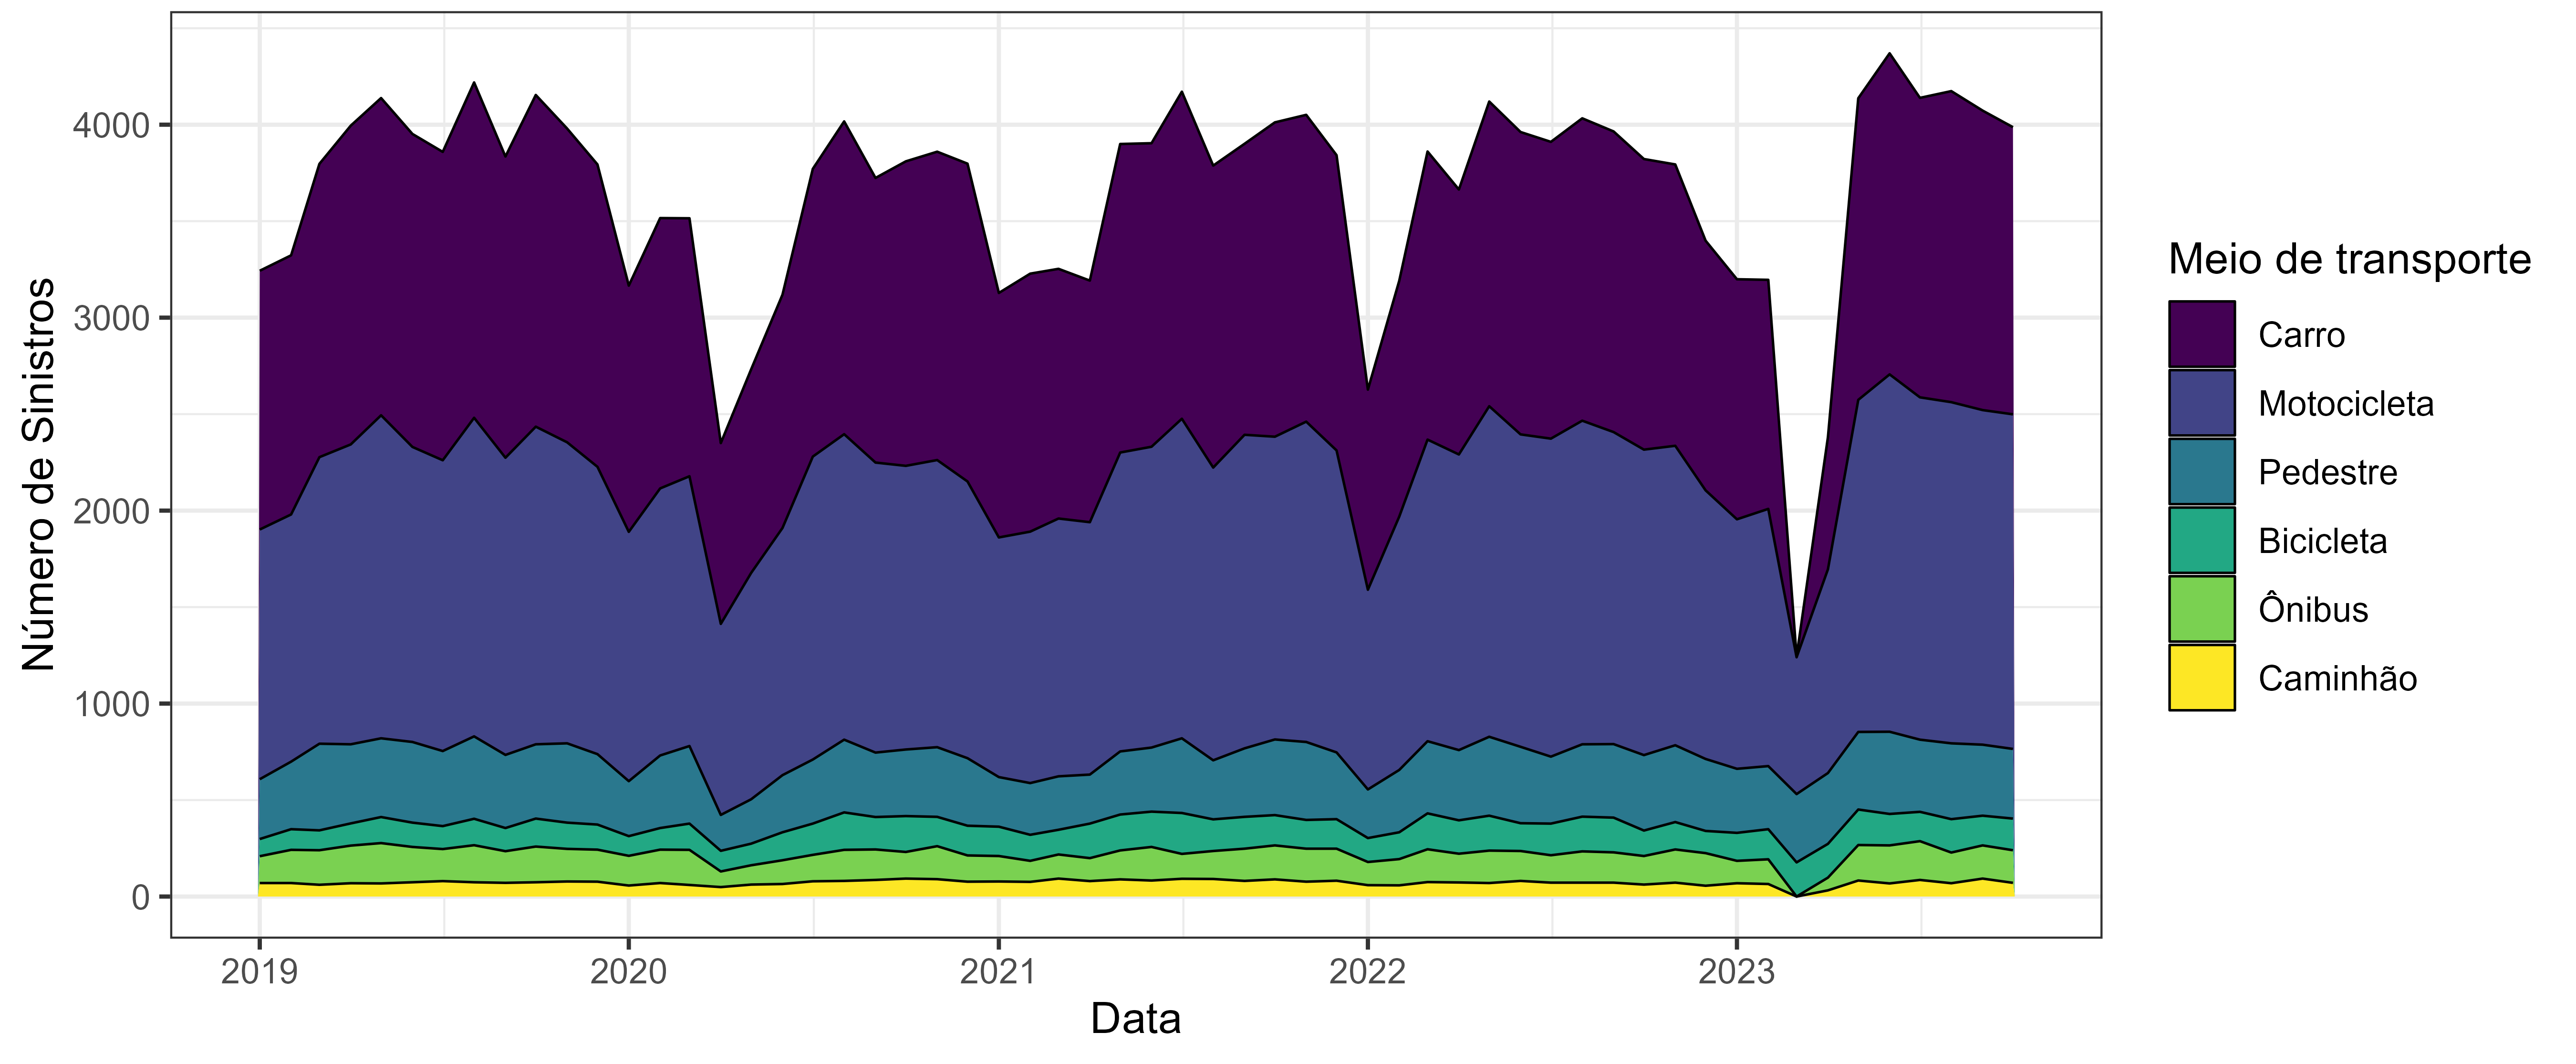
\includegraphics[width = 1\linewidth]{relatorios/faixa-azul/figuras/sinistros_sp.png}
    \label{fig:sinistros}
\end{figure}

Essa intuição tem respaldo da literatura, afinal, a teoria de desenho urbano considera que em vias com usos mistos de automóveis, caminhões, motocicletas, ônibus e bicicletas, a segregação de usos é uma estratégia que pode melhorar o fluxo e segurança dos veículos. \textcite{jun1992traffic} analisam como a segregação de usos entre veículos motorizados e não motorizados ao longo das vias e em intersecções de cidades chinesas reduz o conflito entre eles e, portanto, é importante para garantir maior segurança.

Foi com essa mentalidade que a Companhia de Engenharia de Tráfego (CET), um órgão da Secretaria Municipal de Mobilidade e Trânsito de São Paulo, deu o primeiro passo para implementar essa medida nas vias de SP. Segundo o Código de Trânsito Brasileiro (CTB Art. 80 \S 2), a implementação de uma medida não prevista no código segue a seguinte diretriz: ``O órgão máximo executivo de trânsito da União poderá autorizar, em caráter experimental e por período prefixado, a utilização de sinalização e equipamentos não previstos neste Código''. Portanto, em janeiro de 2022, a CET implementa com cunho experimental a Faixa Azul, uma via exclusiva para motocicletas. A primeira via que recebe essa nova medida é a Avenida 23 de Maio, e é possível observar como fica a divisão das faixas na Figura \ref{fig:23maio}.

\begin{figure}[h]
    \centering
    \caption{Nova disposição da Avenida 23 de Maio}
    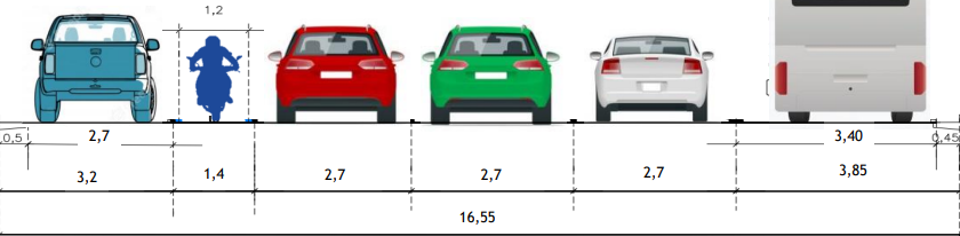
\includegraphics[width = 0.9\linewidth]{relatorios/faixa-azul/figuras/render_faixa_azul.png}
    \label{fig:23maio}
\end{figure}

Entretanto, essa não é a primeira vez que São Paulo experiencia a segregação de usos das vias. A primeira motofaixa no Brasil foi implementada em 2006, na Avenida Sumaré e a segunda, em 2010 na Avenida Vergueiro. Todavia, ambas as faixas foram desativadas em 2013 e 2014, respectivamente. A CET afirma que a faixa foi extinta porque ``não representou aumento da segurança dos motociclistas'' e a decisão de desativar foi elogiada por especialistas (\citefield{noticiaDesativacao}{journaltitle} \citefield{noticiaDesativacao}{year}). De acordo com o \textcite{origemFaixaAzul}, ``[a motofaixa] era à esquerda e um dos motivos de não ter funcionado é que os motociclistas não gostam de andar perto da guia, pois são locais com resíduos e que podem enganchar a pedaleira''.

\begin{figure}[h]
    \caption{Perfil geográfico dos sinistros no município de São Paulo}
    \begin{subfigure}[t]{0.45\linewidth}
        \centering
        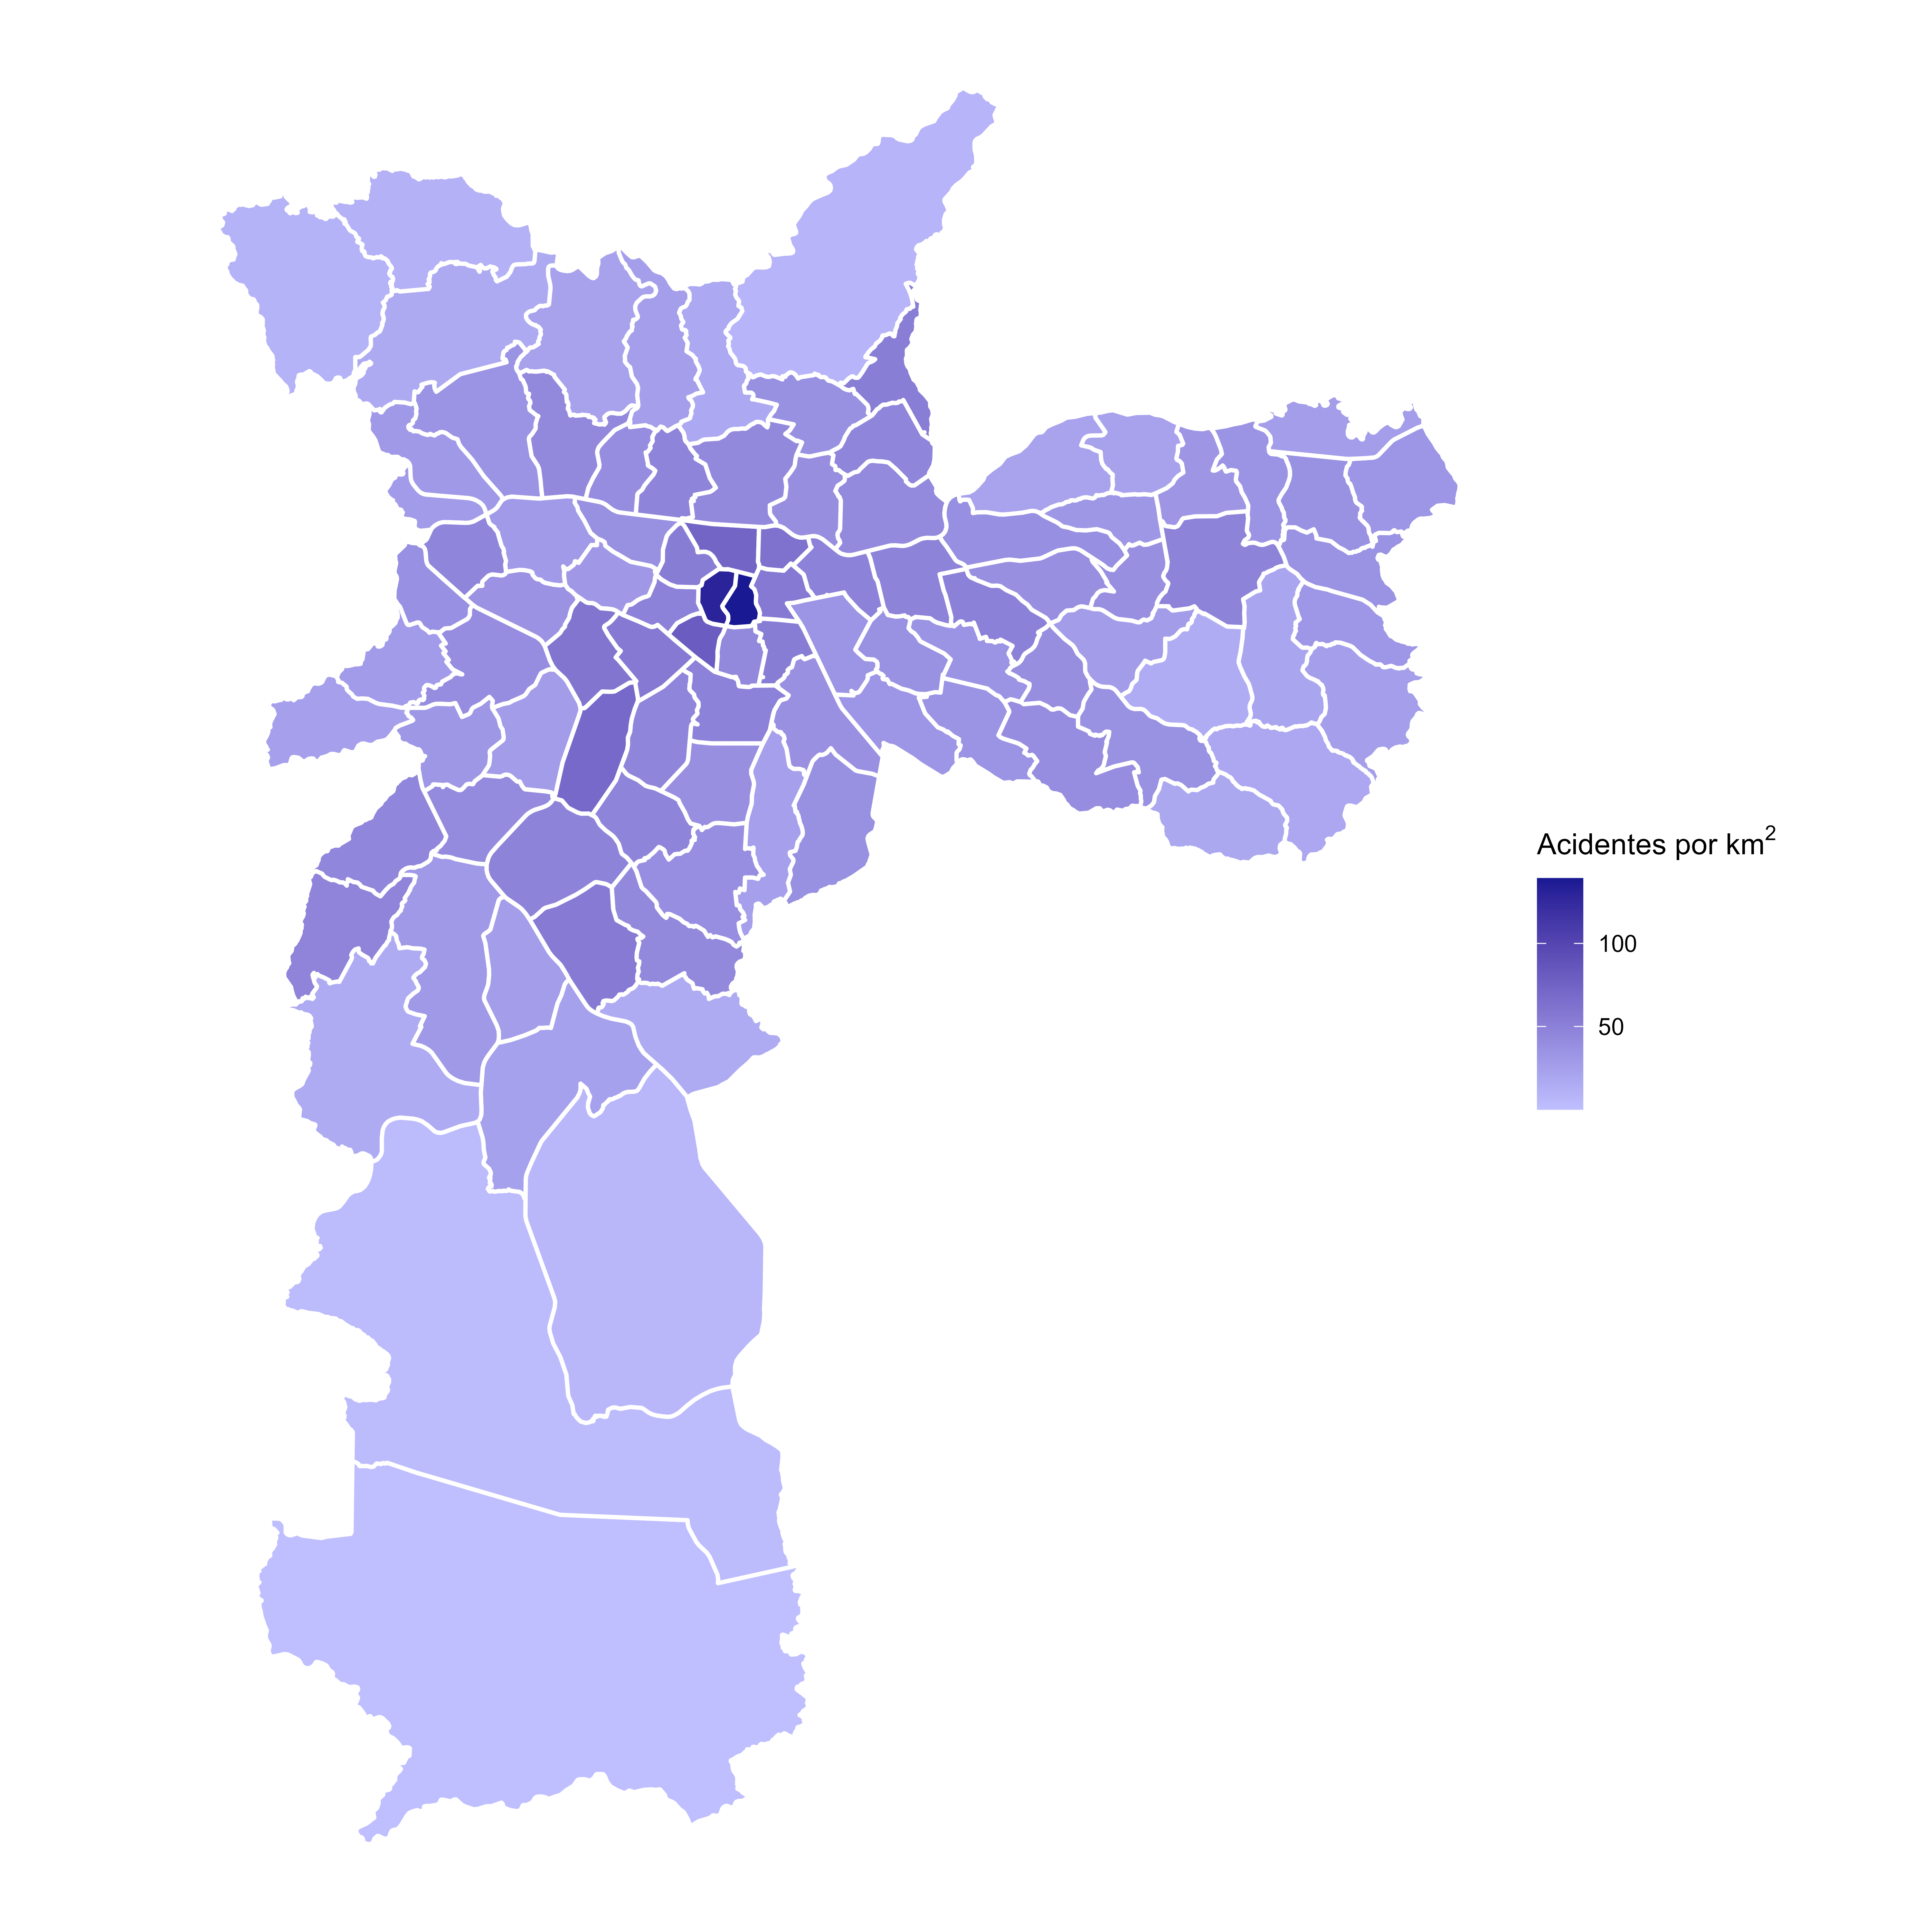
\includegraphics[width = 0.9\linewidth]{relatorios/faixa-azul/figuras/mapa_bairros.png}
        \caption{Distribuição espacial dos sinistros}
        \label{fig:mapa}
    \end{subfigure}
    \hfill
    \begin{subfigure}[t]{0.45\linewidth}
        \centering
        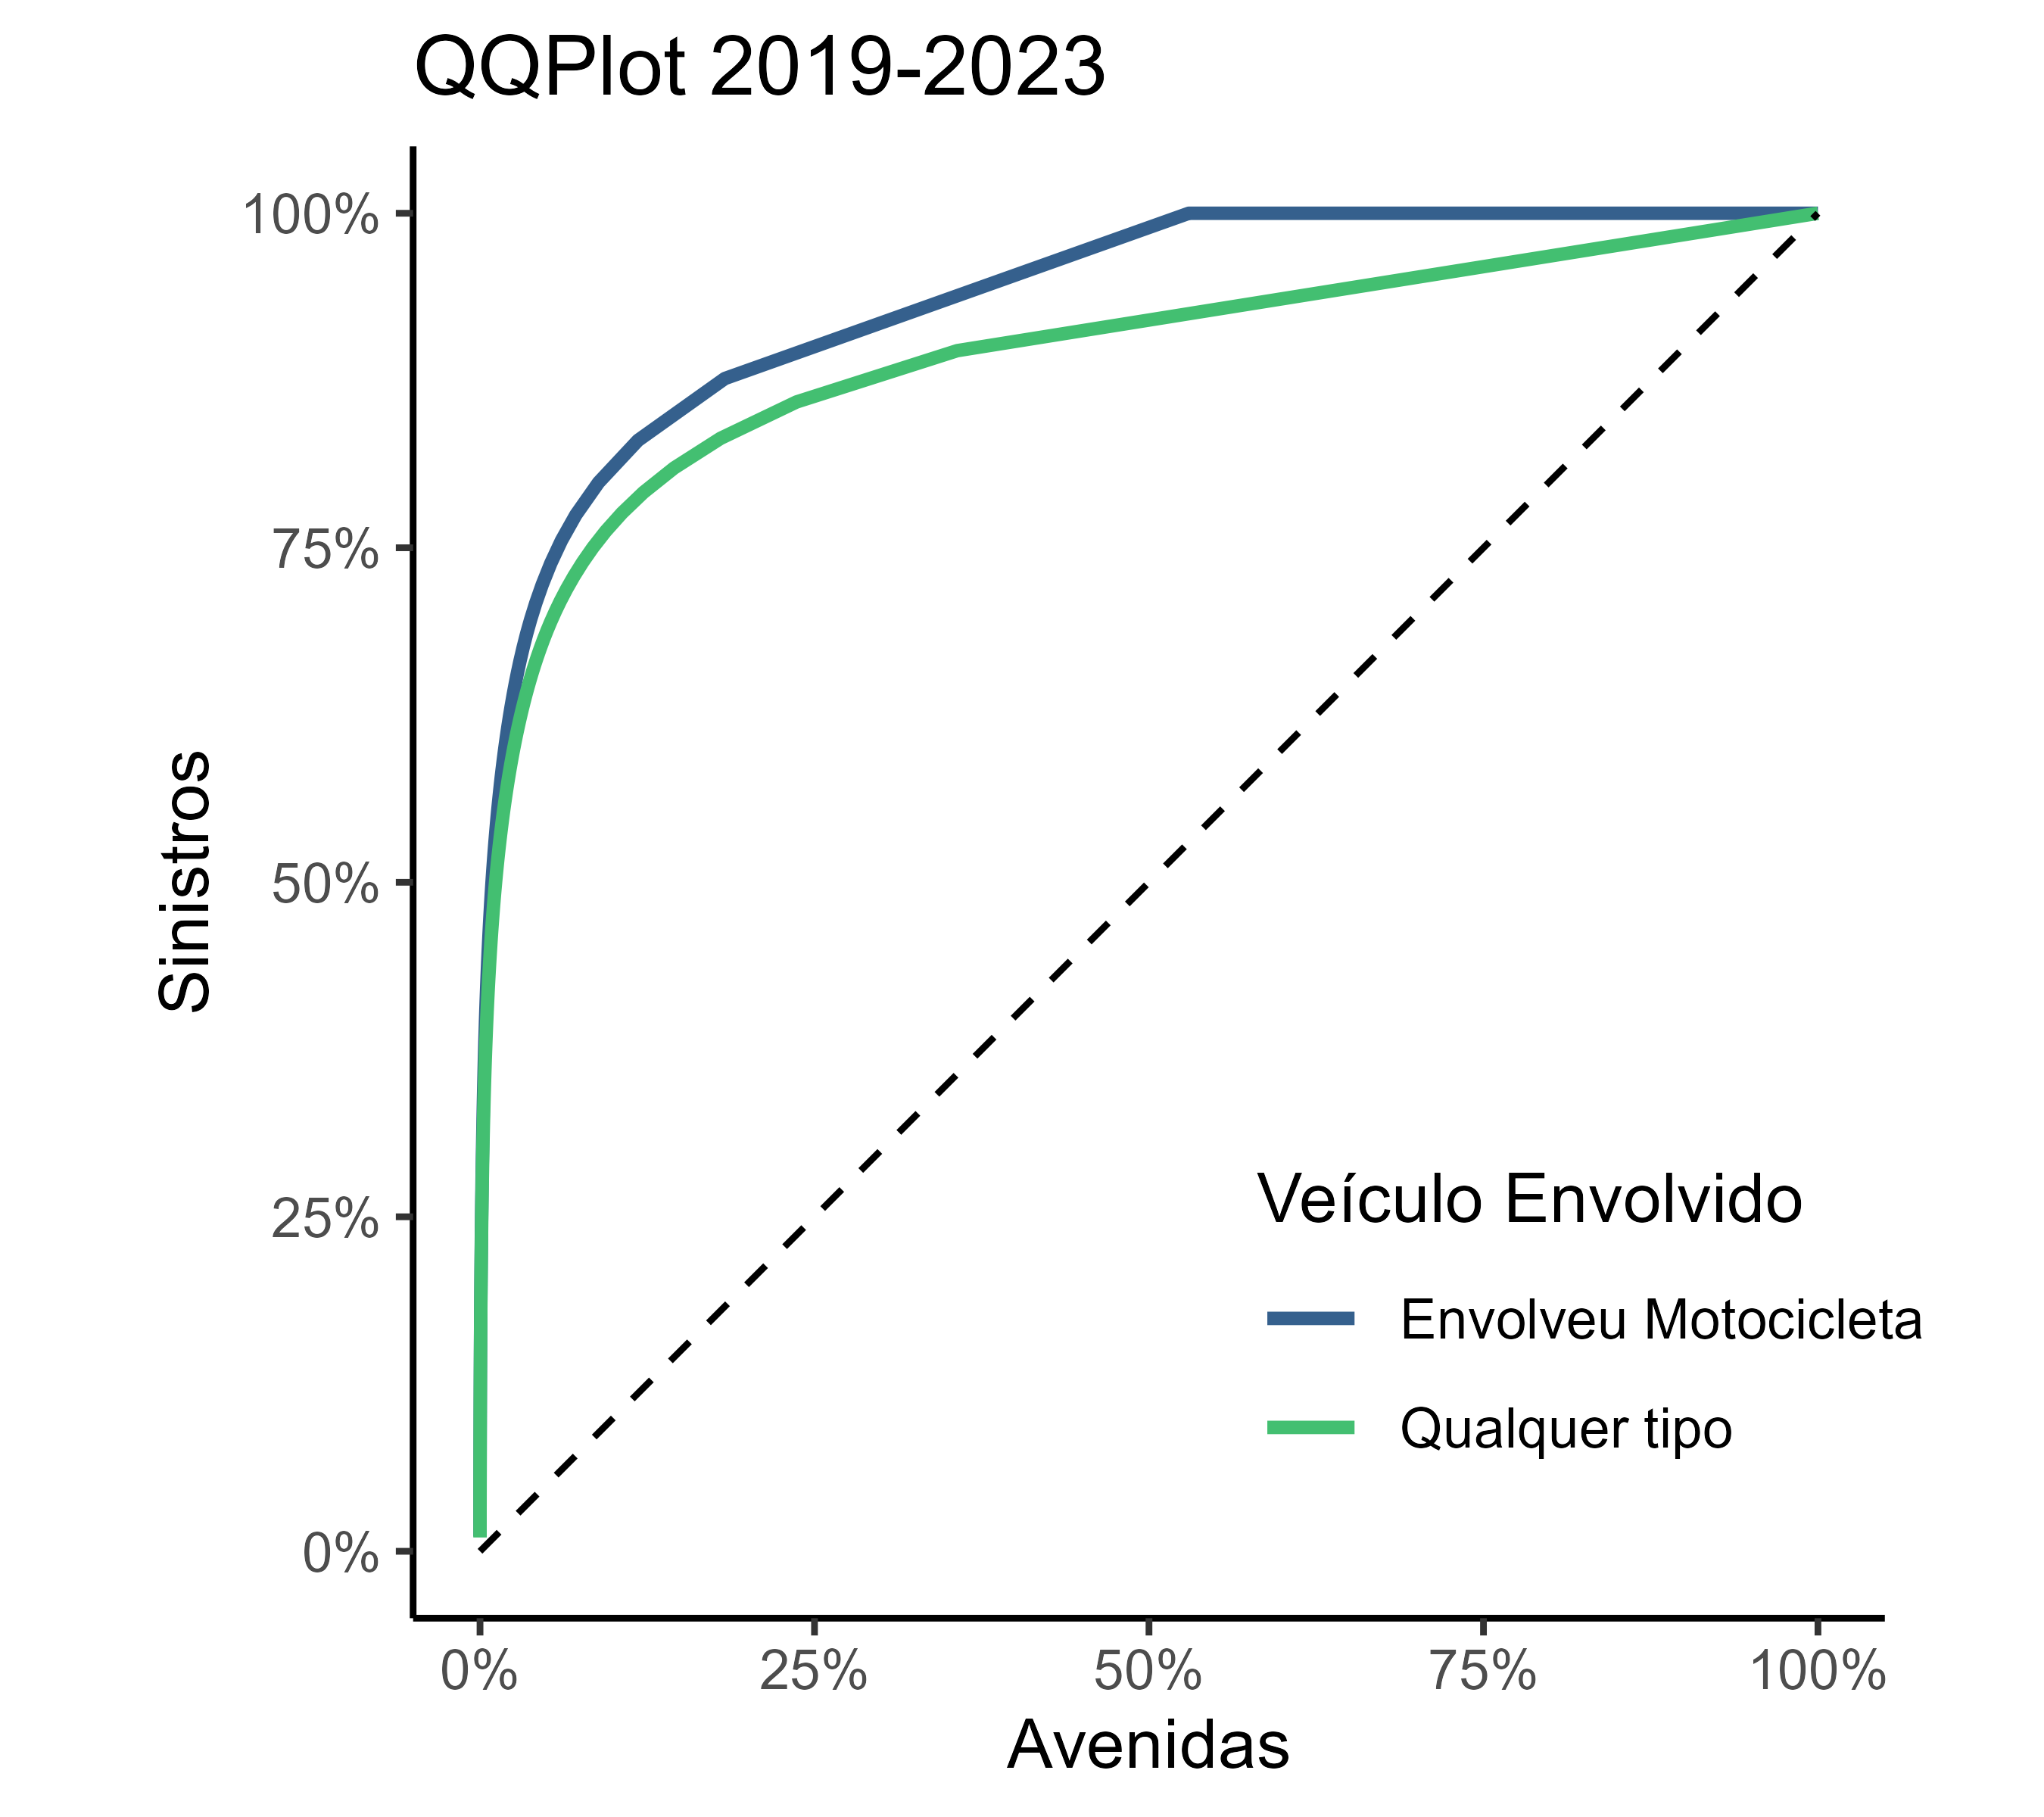
\includegraphics[width = 0.9\linewidth]{relatorios/faixa-azul/figuras/qqplot.png}
        \caption{Concentração dos sinistros (QQ-Plot)}
        \label{fig:qqplot}
    \end{subfigure}
\end{figure}

É importante destacar também o perfil geográfico dos sinistros. O que se pode concluir no caso de São Paulo é que eles estão muito concentrados em grandes avenidas, principalmente nas regiões centrais da cidade, como é possível observar na Figura \ref{fig:mapa}. Na Figura \ref{fig:qqplot}, observa-se que 50\% dos sinistros estão concentrados em menos de 1\% das avenidas. Isso é um indicativo de que caso seja feita uma intervenção bem sucedida nessas poucas e relevantes avenidas, grande parte do problema será resolvido.

Considerando, portanto, tanto o caráter experimental do novo modelo de motofaixa, quanto seu fracasso no passado, é necessária uma análise de seu desempenho para avaliar se deve ser implementada em maior escala. A \textcite{premioSENATRAN} anunciou o sucesso da medida após um ano de faixa azul sem mortes e a iniciativa foi premiada pelo SENATRAN. No entanto, todas as análises feitas foram puramente descritivas e não conferem nenhum tipo de inferência causal, ou seja, não é possivel saber se o efeito analisado foi causado pela faixa azul ou descreve uma relação espúria, uma coincidência. A Avenida 23 de Maio, que teve zero mortes durante o primeiro ano da medida, também apresentou zero mortes em 2019 \cite{relatorioCET}, além de que outros fatores podem interferir na dinâmica do trânsito em São Paulo e precisam ser controlados.

Dessa forma, o presente estudo tem como objetivo investigar se a implementação da faixa azul causou um aumento na segurança viária.
